\documentclass[11pt]{article}

\usepackage[a4paper,margin=1in]{geometry}
\usepackage{amsmath}
\usepackage{booktabs}
\usepackage{float}
\usepackage{graphicx}
\usepackage[hidelinks]{hyperref}

\title{Experimental Results Outline}
\author{}
\date{}

\begin{document}

\maketitle
\tableofcontents

\section{Experimental Results}

This section presents a comprehensive experimental evaluation of the proposed
few-qubit QPP-QNN framework. We first describe the datasets, data splits,
evaluation metrics, baseline methods, and training settings used to ensure a
consistent comparison. We then evaluate the model on the clean synthetic
benchmark and compare it with representative classical approaches and other
quantum model families. Its robustness is further examined under multiple
image corruptions and noise intensities, followed by ablation studies of the
main circuit-design choices. Finally, cross-domain transfer experiments and
executions on quantum hardware are reported to assess the generality and
practical feasibility of the proposed framework.

\subsection{Experimental Setup}
\label{sec:experimental-setup}

All methods were evaluated on a common image-level partition of the synthetic
corner benchmark. The experiments formulate local keypoint detection as binary
classification, where patches associated with L-corners, T-junctions, and
X-junctions constitute the positive class and patches sampled away from any
annotated keypoint constitute the negative class. The following protocol
specifies the dataset construction, quantum input representation, reference
methods, training procedure, and evaluation criteria used in the main
experiments.

\subsubsection{Datasets and Data Splits}

The clean benchmark contains 300 grayscale images of size $64\times64$, with
100 images generated for each of the L-corner, T-junction, and X-junction scene
types. The rendered line width ranges from one to three pixels. To introduce
moderate appearance variation without corrupting the underlying geometry, the
image contrast is sampled from $[0.9,1.1]$ and the brightness offset from
$[-0.02,0.02]$. No additive noise or blur is applied to the clean benchmark.
Although the generator retains the original junction type, all three types are
merged into a single keypoint class in the present binary-detection task.

Each image provides 25 candidate centers from which $9\times9$ patches are
extracted. Five candidates are sampled by jittering the annotated keypoint and
are assigned a positive label, whereas the remaining 20 candidates are sampled
at least five pixels away from every annotated keypoint and are assigned a
negative label. The resulting dataset therefore contains 7,500 patches, with
1,500 positive and 6,000 negative examples. Images, rather than individual
patches, are partitioned in order to prevent patches from the same scene from
appearing in different subsets. The split is stratified by scene type and uses
180 images for training, 60 for validation, and 60 for testing, corresponding
to 4,500/1,500/1,500 patches and 900/300/300 positive samples, respectively.
Dataset generation and splitting use random seed 37. All corrupted test sets
in the robustness experiments are derived from the held-out test images while
preserving their candidate centers and labels.

\subsubsection{Model and Quantum Encoding}

For each patch, image gradients are used to form the local structure tensor
\begin{equation}
    \mathbf{M}=
    \begin{bmatrix}
        \sum I_x^2 & \sum I_x I_y \\
        \sum I_x I_y & \sum I_y^2
    \end{bmatrix},
\end{equation}
whose ordered eigenvalues are denoted by $\lambda_1\geq\lambda_2$. We also use
the total structural energy $S=\lambda_1+\lambda_2$ and the normalized
two-directional response
\begin{equation}
    \eta=\frac{4\lambda_1\lambda_2}{(\lambda_1+\lambda_2)^2+\epsilon}.
\end{equation}
The main two-qubit QPP--QNN directly encodes
$[\lambda_1,\lambda_2]$, while the one-qubit variant uses the compact scalar
$t=\log(S+\epsilon)+4\eta$. These representations compress the local
second-order geometry before quantum processing instead of assigning one qubit
to every handcrafted feature.

Feature normalization is fitted exclusively on the training split. For a raw
feature $x_j$, the rotation angle is computed as
\begin{equation}
    z_j=\operatorname{clip}\!\left(
        \frac{x_j-\mu_j}{\sigma_j+\epsilon},-3,3
    \right),
    \qquad
    \phi_j=\frac{\pi}{3}z_j,
\end{equation}
and the same training statistics are then applied to the validation and test
sets. The QPP--QNNs use two data-reuploading layers. Each layer applies
$R_Y(\phi_j)R_Z(\phi_j)$ encoding followed by trainable
$R_ZR_YR_Z$ rotations. The two-qubit model additionally applies a
$\mathrm{CNOT}(0\!\rightarrow\!1)$ gate and measures
$\langle Z_0\rangle$, $\langle Z_1\rangle$, and
$\langle Z_0Z_1\rangle$; the one-qubit model measures $\langle Z\rangle$.
A trainable affine readout followed by a sigmoid maps these expectation values
to the keypoint probability. Unless explicitly stated otherwise, circuit
expectations are evaluated exactly with the differentiable state-vector
simulator, without finite-shot sampling.

\subsubsection{Compared Methods and Training Settings}

The reference methods cover three complementary groups. First, Harris, FAST,
and ORB are included as conventional image-level keypoint detectors. Harris is
run with block size 2, Sobel aperture 3, $k=0.04$, and a relative response
threshold of 0.01; FAST uses threshold 20 with non-maximum suppression; and
each detector retains at most 40 points per image. Second, the classical
learning reference is a multilayer perceptron with hidden widths 32 and 16,
ReLU activations, and the five-dimensional structure-tensor input
$[I_x,I_y,\lambda_1,\lambda_2,R]$. Scalar $\lambda_2$ thresholding and logistic
regression on $[\log(S+\epsilon),\eta]$ are also retained as compact controls.
Third, the quantum comparison includes the proposed one- and two-qubit
QPP--QNNs as well as the earlier feature-dimension-matched QNN families used in
the ablation study.

The MLP is standardized using training-set statistics and optimized with Adam
for at most 300 iterations, using a learning rate of 0.003 and a batch size of
128. The QPP--QNN models are trained on CPU using Adam, a learning rate of 0.01,
a batch size of 128, and at most 40 epochs. A class-weighted binary
cross-entropy loss compensates for the 1:4 positive-to-negative ratio, and
early stopping with patience 8 monitors validation PR-AUC. QPP--QNN training
uses random seed 47. For the QPP--QNNs and compact score-based controls, the
decision threshold is selected on the validation split by maximizing F1 and is
then fixed before evaluating the test split. The archived MLP reference uses
the conventional probability threshold of 0.5. Configuration changes made for
individual noise, low-sample, ablation, or hardware experiments are stated in
their corresponding subsections.

\subsubsection{Evaluation Metrics}
\label{sec:metrics}

Because only 20\% of the candidate patches are positive, accuracy alone can
overstate performance. We therefore use F1 and precision--recall area under the
curve (PR-AUC) as the primary measures and report precision and recall to show
the false-positive/false-negative trade-off. With true positives $TP$, false
positives $FP$, and false negatives $FN$, these metrics are
\begin{equation}
    \mathrm{Precision}=\frac{TP}{TP+FP},
    \qquad
    \mathrm{Recall}=\frac{TP}{TP+FN},
\end{equation}
and
\begin{equation}
    F_1=2\frac{\mathrm{Precision}\cdot\mathrm{Recall}}
    {\mathrm{Precision}+\mathrm{Recall}}.
\end{equation}
PR-AUC is implemented as average precision rather than trapezoidal
interpolation. For operating points indexed in descending score order, it is
computed as
\begin{equation}
    \mathrm{PR\mbox{-}AUC}
    =\mathrm{AP}
    =\sum_n\left(R_n-R_{n-1}\right)P_n,
\end{equation}
where $P_n$ and $R_n$ denote precision and recall at the $n$th threshold.
Accuracy and ROC-AUC are retained as secondary diagnostics. Patch classifiers
are scored at the candidate level. For the conventional image detectors, a
detected point is counted as a true positive when it can be uniquely matched
to an unmatched ground-truth keypoint within a three-pixel tolerance; all
remaining detections and annotations are counted as false positives and false
negatives, respectively.

\subsection{Main Results on the Clean Benchmark}
\label{sec:clean-main-results}

We first examine whether the compact phase-coordinate QPP--QNN retains enough
local geometric information to distinguish keypoints from non-keypoints under
clean imaging conditions. The comparison includes three conventional
full-image detectors, a shared-feature MLP, and the proposed one- and
two-qubit QPP--QNNs. Table~\ref{tab:clean-main-results} reports the complete
clean-test metrics, while Fig.~\ref{fig:clean-test-f1} provides a direct visual
comparison of their F1 scores.

\subsubsection{Overall Clean-Test Comparison}

\begin{table}[H]
    \centering
    \caption{Clean synthetic corner/junction results for the classical
    references and phase-coordinate QPP--QNNs.}
    \label{tab:clean-main-results}
    \small
    \begin{tabular}{llcccc}
        \toprule
        Method & Input & Precision & Recall & F1 & PR-AUC \\
        \midrule
        Harris & image & 0.1652 & 0.9500 & 0.2815 & 0.8953 \\
        FAST & image & 0.0789 & 0.7833 & 0.1433 & 0.7925 \\
        ORB & image & 0.0412 & 1.0000 & 0.0791 & 0.7759 \\
        MLP & shared 5D features & \textbf{0.9347} & 0.9067 & 0.9205 & \textbf{0.9749} \\
        QPP--QNN 1q L2 & scalar-$c4$ & 0.8679 & \textbf{0.9633} & 0.9131 & 0.9437 \\
        QPP--QNN 2q L2 & $[\lambda_1,\lambda_2]$ & 0.8865 & \textbf{0.9633} & \textbf{0.9233} & 0.9448 \\
        \bottomrule
    \end{tabular}
\end{table}

The two groups in Table~\ref{tab:clean-main-results} use related but distinct
operating protocols. For Harris, FAST, and ORB, precision, recall, and F1 are
obtained by one-to-one spatial matching within three pixels, whereas PR-AUC is
computed by ranking their response values at the sampled candidate centers.
For the MLP and QPP--QNNs, all metrics are computed directly from candidate
classification scores. The full-image detectors should therefore be regarded
as operational image references rather than parameter- or input-matched
learners. Comparisons within the learned-model group are more direct because
these models are evaluated on the same local candidates and image-level split.

\begin{figure}[H]
    \centering
    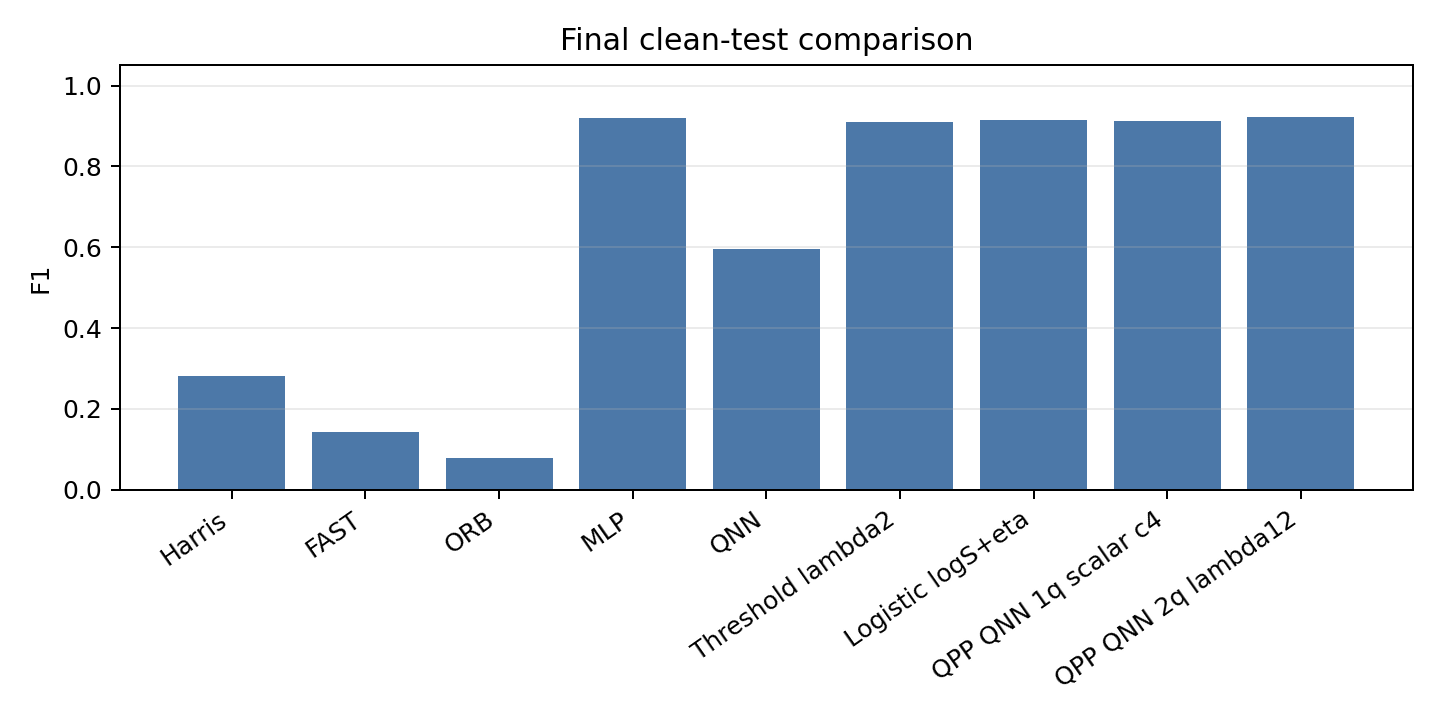
\includegraphics[width=\linewidth]{../outputs/summaries/final_comparison_results.png}
    \caption{Clean-test F1 comparison among the full-image classical detectors
    (Harris, FAST, and ORB), the shared-feature MLP, and the one- and two-qubit
    phase-coordinate QPP--QNNs. The classical detectors are evaluated by
    spatial point matching, whereas the learned models classify the same
    sampled local candidates.}
    \label{fig:clean-test-f1}
\end{figure}

Figure~\ref{fig:clean-test-f1} shows a clear separation between the conventional
detectors and the learned local classifiers on this sparse geometric benchmark.
It also shows that both few-qubit models operate in the same F1 regime as the
MLP despite using only one or two geometric coordinates as quantum inputs.
The following comparisons examine these two observations in more detail.

\subsubsection{Comparison with Classical References}

Among the full-image detectors, Harris gives the strongest F1 score of 0.2815,
followed by FAST at 0.1433 and ORB at 0.0791. Their recalls remain relatively
high---0.9500, 0.7833, and 1.0000, respectively---but their precisions fall to
0.1652, 0.0789, and 0.0412. Thus, these methods locate most annotated
junctions but also produce many unmatched responses on the sparse line
drawings. This behavior is consistent with their local response rules: strong
gradient changes can generate detections even when the response does not
correspond to the labeled candidate geometry.

The MLP is a substantially stronger classical learning reference. Using the
shared five-dimensional structure-tensor features, it reaches 0.9347 precision,
0.9067 recall, 0.9205 F1, and 0.9749 PR-AUC. Its high PR-AUC indicates that its
scores rank positive candidates consistently over a wide range of decision
thresholds. The large gap between the MLP and the full-image detectors should
not, however, be attributed solely to the model family: the MLP benefits from
candidate-level supervision, while Harris, FAST, and ORB operate directly on
the image without access to the learned patch labels. The MLP therefore serves
as the principal classical comparator for judging the learned QPP models.

\subsubsection{Comparison between One- and Two-Qubit QPP Models}

The one-qubit QPP--QNN compresses the local spectrum into
$t=\log(S+\epsilon)+4\eta$ and achieves 0.8679 precision, 0.9633 recall,
0.9131 F1, and 0.9437 PR-AUC with two re-uploading layers. This result shows
that a single-qubit circuit driven by one geometry-informed scalar already
captures a useful keypoint decision boundary. The two-qubit model instead
retains the ordered eigenvalues $[\lambda_1,\lambda_2]$ as separate phase
coordinates. It preserves the same 0.9633 recall while increasing precision to
0.8865, which raises F1 to 0.9233. Relative to the one-qubit model, this is an
absolute F1 improvement of 0.0102, whereas PR-AUC changes only slightly from
0.9437 to 0.9448. The improvement is therefore mainly associated with a better
fixed operating point rather than a large change in global score ranking.

Compared with the MLP, the archived two-qubit result has a marginally higher
F1 (0.9233 versus 0.9205) and higher recall (0.9633 versus 0.9067), but lower
precision (0.8865 versus 0.9347) and lower PR-AUC (0.9448 versus 0.9749).
Moreover, as described in Section~\ref{sec:experimental-setup}, the archived
MLP uses a threshold of 0.5, whereas the QPP--QNN threshold is selected on the
validation split. We therefore interpret the result as evidence that a shallow
two-qubit phase-coordinate model is competitive with the classical learner at
the selected operating point, rather than as evidence of an overall quantum
advantage. Its main benefit in this experiment is resource efficiency: the
model retains strong clean-test detection performance using two qubits, two
re-uploading layers, and a compact spectral input.

\subsection{Separating L-Corners, T-Junctions, and X-Junctions}
\label{sec:ltx-multiclass}

The binary benchmark in Section~\ref{sec:clean-main-results} treats L-corners,
T-junctions, and X-junctions as a single positive keypoint class. We next ask
whether the same local structure-tensor representation retains enough
geometric information to distinguish these three structures from one another.
This experiment is therefore a three-class classification task conditioned on
patches that contain an annotated keypoint; it is not a four-class detector
with an additional background category. Besides testing finer geometric
semantics, this setting allows a compact classical--quantum comparison under a
common input representation and a group-disjoint evaluation protocol.

\subsubsection{Multiclass Protocol and Evaluation Metrics}

The dataset contains 120 independently rendered source-image groups for each
of the L-, T-, and X-junction classes. Four positive patches are sampled from
each group, yielding $120\times4\times3=1{,}440$ labeled patches in total. A
stratified 60/20/20 split is performed at the source-group level, resulting in
864 training, 288 validation, and 288 test patches. Group-level separation is
essential because patches derived from the same rendered source can share
nearly identical geometry and appearance; allowing them to cross subsets would
therefore lead to an overly optimistic estimate of generalization.

All learners receive the same eight-dimensional structure-tensor interface,
\begin{equation}
    \mathbf{x}=
    [I_x,I_y,I_x^2,I_y^2,I_xI_y,\lambda_1,\lambda_2,R],
\end{equation}
and feature normalization is fitted only on the training split. Results are
aggregated over five training seeds. For models that are retrained for every
seed, we report the sample mean and standard deviation; deterministic reference
values are reported once when no run-to-run variation is available.

Because the task contains three target classes, we use macro averages. For a
class $c\in\{L,T,X\}$, that class is treated as
positive and the other two as negative, giving
\begin{equation}
    P_c=\frac{TP_c}{TP_c+FP_c},
    \qquad
    R_c=\frac{TP_c}{TP_c+FN_c},
    \qquad
    F_{1,c}=2\frac{P_cR_c}{P_c+R_c}.
\end{equation}
Macro-F1 assigns equal importance to the three geometric categories:
\begin{equation}
    \mathrm{Macro\mbox{-}F1}
    =\frac{1}{3}\sum_{c\in\{L,T,X\}}F_{1,c}.
\end{equation}
Likewise, a one-vs-rest precision--recall curve is constructed for each class,
and the three classwise areas are averaged:
\begin{equation}
    \mathrm{Macro\mbox{-}PR\mbox{-}AUC}
    =\frac{1}{3}\sum_{c\in\{L,T,X\}}
    \mathrm{PR\mbox{-}AUC}_c.
\end{equation}
These macro averages prevent performance on one comparatively easy class from
dominating the reported score and directly assess whether a model recognizes
all three junction types consistently.

\subsubsection{Compared Classical and Quantum Models}

Four models are compared under the shared feature and split protocol. The
multinomial logistic model is the linear reference, with class probabilities
\begin{equation}
    \mathbf{p}(y\mid\mathbf{x})
    =\operatorname{softmax}(\mathbf{W}\mathbf{x}+\mathbf{b}).
\end{equation}
For eight inputs and three output classes, it contains
$8\times3+3=27$ trainable parameters and measures the linear separability of
the junction types. The RBF SVM supplies a stronger nonlinear classical
reference through the kernel
\begin{equation}
    K(\mathbf{x}_i,\mathbf{x}_j)
    =\exp\!\left(-\gamma\lVert\mathbf{x}_i-\mathbf{x}_j\rVert_2^2\right).
\end{equation}
Its complexity depends on the selected support vectors, so it is listed as
nonparametric rather than assigned a fixed parameter count.

TinyMLP h5 uses a single hidden layer of width five between the eight inputs
and the three-class output. Its parameter count is
\begin{equation}
    (8\times5+5)+(5\times3+3)=63,
\end{equation}
making it a compact nonlinear neural baseline. The quantum comparator is a
four-qubit, two-layer grouped data-reuploading QNN with 67 trainable parameters.
Across its two layers, the eight input coordinates are distributed over four
qubits, followed by trainable local rotations, ring entanglers, Pauli readout,
and an affine three-class head. The 63-parameter TinyMLP and 67-parameter QNN
therefore provide an approximately parameter-matched classical--quantum
comparison, although their computational primitives remain fundamentally
different.

\subsubsection{Results and Discussion}

\begin{table}[H]
    \centering
    \caption{Three-class L/T/X classification under a source-image-disjoint
    split. Neural and kernel results are aggregated over five seeds.}
    \label{tab:ltx-multiclass}
    \begin{tabular}{lccc}
        \toprule
        Model & Parameters & Macro-F1 & Macro PR-AUC \\
        \midrule
        Multinomial logistic & 27 & 0.7719 & 0.7942 \\
        RBF SVM & nonparametric & $0.7700\pm0.0018$ & $\mathbf{0.8656\pm0.0004}$ \\
        TinyMLP h5 & 63 & $\mathbf{0.8077\pm0.0238}$ & $0.8206\pm0.0140$ \\
        Grouped QNN 4q L2 & 67 & $0.7636\pm0.0232$ & $0.7934\pm0.0122$ \\
        \bottomrule
    \end{tabular}
\end{table}

\begin{figure}[H]
    \centering
    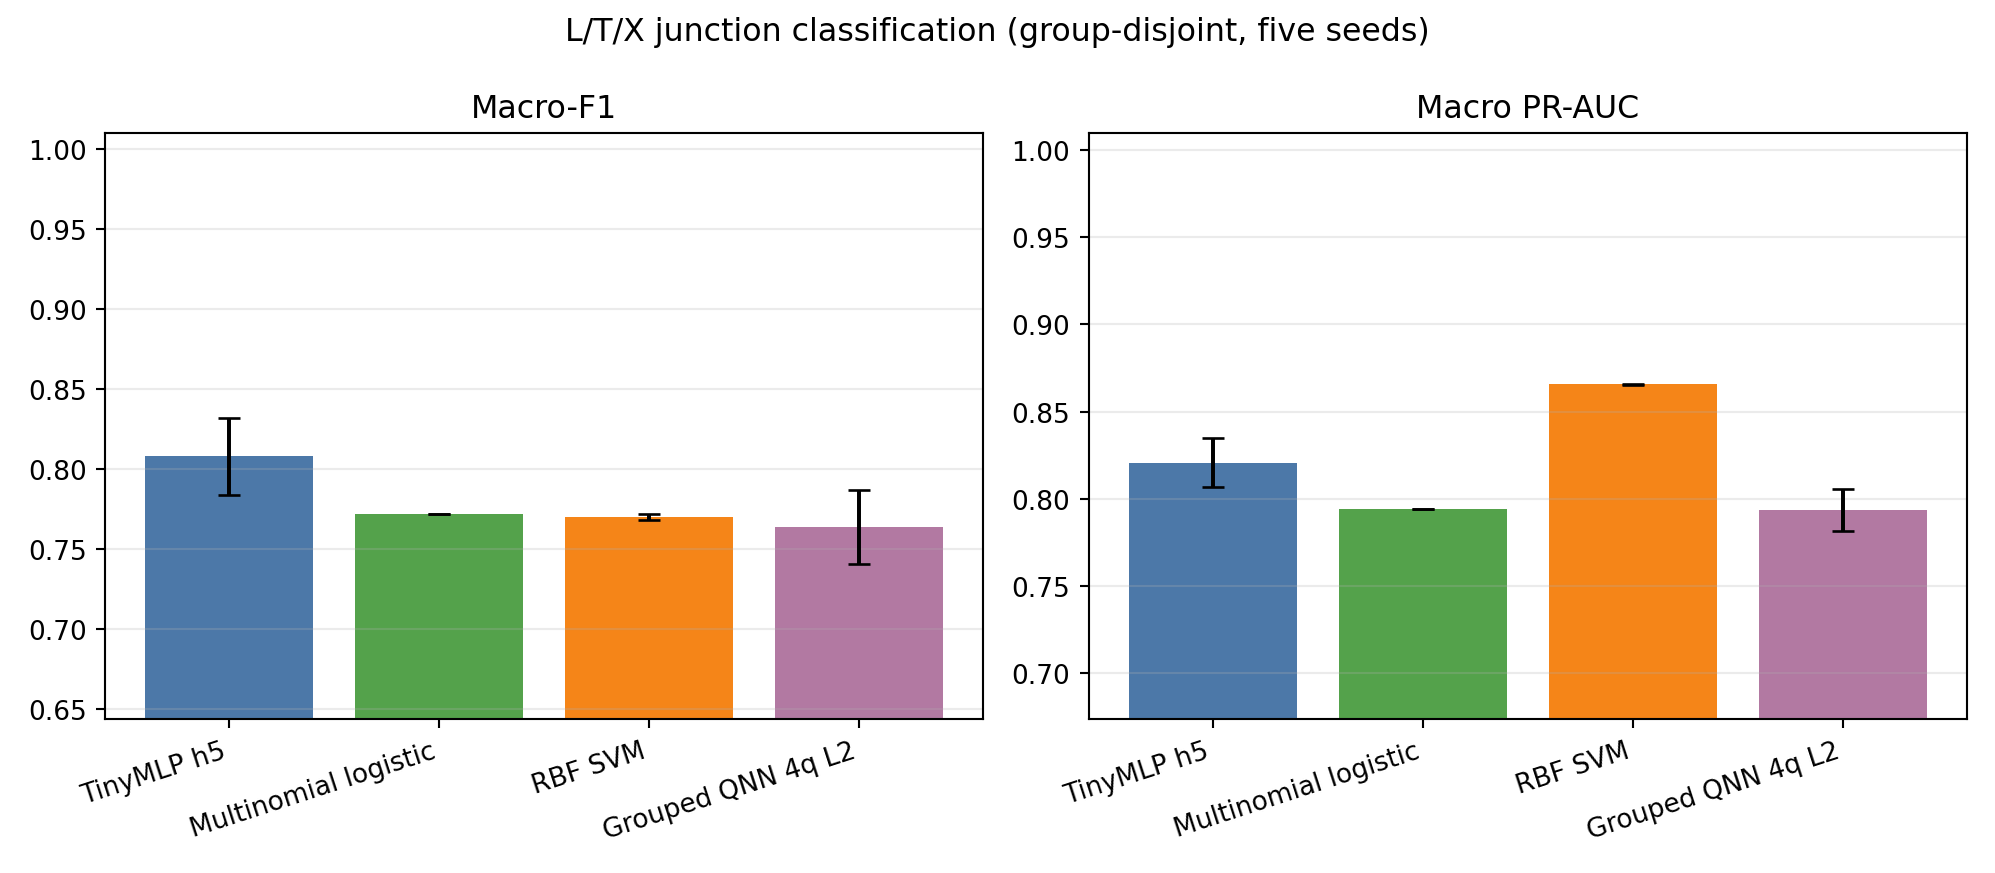
\includegraphics[width=\linewidth]{../missing_draft_figures/Figure_05_ltx_multiclass_comparison.png}
    \caption{Five-seed L/T/X classification under a group-disjoint split. Bars
    show mean Macro-F1 and Macro PR-AUC, and error bars show standard deviations
    where repeated-run estimates are available. TinyMLP achieves the highest
    Macro-F1, whereas the RBF SVM achieves the highest Macro PR-AUC.}
    \label{fig:ltx-multiclass}
\end{figure}

As shown in Table~\ref{tab:ltx-multiclass} and
Fig.~\ref{fig:ltx-multiclass}, TinyMLP gives the best final classification
balance, reaching a Macro-F1 of $0.8077\pm0.0238$. Its advantage over
multinomial logistic regression indicates that the junction types are not
fully separated by linear decision boundaries in the shared eight-dimensional
feature space. The RBF SVM attains a lower Macro-F1 of
$0.7700\pm0.0018$ but the highest Macro PR-AUC of
$0.8656\pm0.0004$. It therefore provides the most consistent one-vs-rest score
ranking across the three classes, with very little variation across runs, even
though its final multiclass decisions do not maximize Macro-F1.

The grouped four-qubit QNN reaches $0.7636\pm0.0232$ Macro-F1 and
$0.7934\pm0.0122$ Macro PR-AUC. These values demonstrate nontrivial learning
of L/T/X geometry and are close to the 27-parameter multinomial logistic
reference, but they remain below the best classical results. In particular,
the approximately parameter-matched TinyMLP exceeds the QNN by 0.0441 in
Macro-F1, while the RBF SVM exceeds it by 0.0722 in Macro PR-AUC. The present
experiment therefore supports task extensibility rather than quantum
superiority: the local PSD representation and grouped QNN can be extended from
binary keypoint presence to finer junction semantics, but the classical
TinyMLP and RBF SVM remain stronger under the current protocol. This outcome
also motivates the controlled quantum-family study in the next subsection,
where the input, qubit count, training budget, and threshold protocol are held
fixed more tightly.

\subsection{Few-Qubit Quantum-Family Comparison}
\label{sec:quantum-family}

Having established the feasibility of spectrum-based quantum classification,
we next ask a more focused question: which quantum encoding and circuit family
offers the most favorable performance under the same small-qubit budget?  This
experiment is an intra-quantum comparison rather than a claim of quantum
advantage.  Its purpose is to separate the effects of state preparation,
variational-circuit structure, and parameter count while keeping the classical
input and evaluation procedure fixed.

\subsubsection{Controlled Comparison Protocol}

All models receive the same ordered tensor-spectrum feature
$\boldsymbol{x}=[\lambda_1,\lambda_2]$, use the same image-level train/validation/test
split and feature normalization, and are evaluated on the same clean test set.
The trainable circuits use two qubits and two variational layers.  We also hold
the optimizer, training budget, and validation-based threshold-selection rule
fixed.  F1 and PR-AUC are computed using the definitions in
Section~\ref{sec:metrics}; the reported values are the mean and standard
deviation over multiple random seeds.  Consequently, the comparison reflects
differences among the quantum model families rather than changes in data
partitioning or evaluation protocol.

The two fidelity-kernel baselines shown in Fig.~\ref{fig:quantum-family} use
the same inputs and split, but they are not variational QNNs.  They construct a
fixed quantum similarity matrix and pass it to a classical kernel learner.
They are therefore included as references in the figure, but excluded from the
trainable-parameter comparison in Table~\ref{tab:quantum-family}.

\subsubsection{Quantum Model Families}

The comparison covers complementary ways of embedding and processing the two
spectral coordinates:

\begin{itemize}
    \item \textbf{Schmidt-QPP QNN.}  The normalized spectrum
    $\mu_i=\lambda_i/(\lambda_1+\lambda_2)$ is encoded as the amplitudes of a
    correlated two-qubit state,
    \begin{equation}
        \lvert\psi_{\mathrm{S}}(\boldsymbol{x})\rangle
        =\sqrt{\mu_1}\lvert 00\rangle+\sqrt{\mu_2}\lvert 11\rangle.
        \label{eq:schmidt-encoding}
    \end{equation}
    A shallow parameterized circuit and Pauli-expectation readout then learn
    the decision function.  This construction places the relative local
    spectrum directly in a correlated subspace.

    \item \textbf{Data re-uploading QNN.}  The normalized coordinates are
    repeatedly injected as single-qubit rotation angles at every layer, with
    trainable local rotations and a shallow entangling operation between
    successive uploads.  Repeated access to the data can increase the
    nonlinearity of a shallow circuit without increasing the qubit count.

    \item \textbf{HEA-VQC with angle encoding.}  A conventional
    hardware-efficient ansatz combines angle encoding, trainable local
    rotations, and shallow two-qubit entanglers.  It provides a generic
    variational baseline that is not tailored specifically to the tensor
    spectrum.

    \item \textbf{Separable VQC with angle encoding.}  This control retains
    local angle encoding and trainable one-qubit transformations but removes
    the two-qubit entangling operation.  Its comparison with the entangling
    circuits tests whether independent processing of $\lambda_1$ and
    $\lambda_2$ is sufficient under the same shallow-depth regime.

    \item \textbf{IQP-VQC.}  This model uses an IQP-style phase feature map
    followed by a trainable variational readout.  It tests whether a
    phase-interaction encoding is well matched to the ordered spectral input.
\end{itemize}

For completeness, the two fixed quantum-kernel references use either an
IQP-based feature state or the Schmidt state in
Eq.~\eqref{eq:schmidt-encoding}.  Their kernel entries are
\begin{equation}
    K(\boldsymbol{x}_i,\boldsymbol{x}_j)
    =\left|\left\langle\psi(\boldsymbol{x}_i)
      \middle|\psi(\boldsymbol{x}_j)\right\rangle\right|^2,
    \label{eq:fidelity-kernel}
\end{equation}
so their learnable decision boundary is produced by the classical kernel
learner rather than by optimizing quantum-circuit parameters.

\subsubsection{Results and Resource--Performance Trade-offs}

\begin{table}[H]
    \centering
    \caption{Controlled comparison of trainable two-qubit model families on
    the clean test set.  Results are reported as mean $\pm$ standard deviation
    over multiple random seeds.  Bold entries denote the best value in each
    metric.}
    \label{tab:quantum-family}
    \small
    \begin{tabular}{lccc}
        \toprule
        Model & Trainable parameters & F1 & PR-AUC \\
        \midrule
        Schmidt-QPP QNN, $L=2$       & 25 & $\mathbf{0.9279\pm0.0045}$ & $0.9539\pm0.0065$ \\
        Data re-uploading QNN, $L=2$ & 16 & $0.9181\pm0.0099$ & $0.9470\pm0.0072$ \\
        HEA-VQC angle, $L=2$         & 16 & $0.9179\pm0.0088$ & $\mathbf{0.9650\pm0.0025}$ \\
        Separable VQC angle, $L=2$   & 16 & $0.8961\pm0.0080$ & $0.9540\pm0.0061$ \\
        IQP-VQC, $L=2$               & 16 & $0.8574\pm0.0404$ & $0.9092\pm0.0338$ \\
        \bottomrule
    \end{tabular}
\end{table}

\begin{figure}[H]
    \centering
    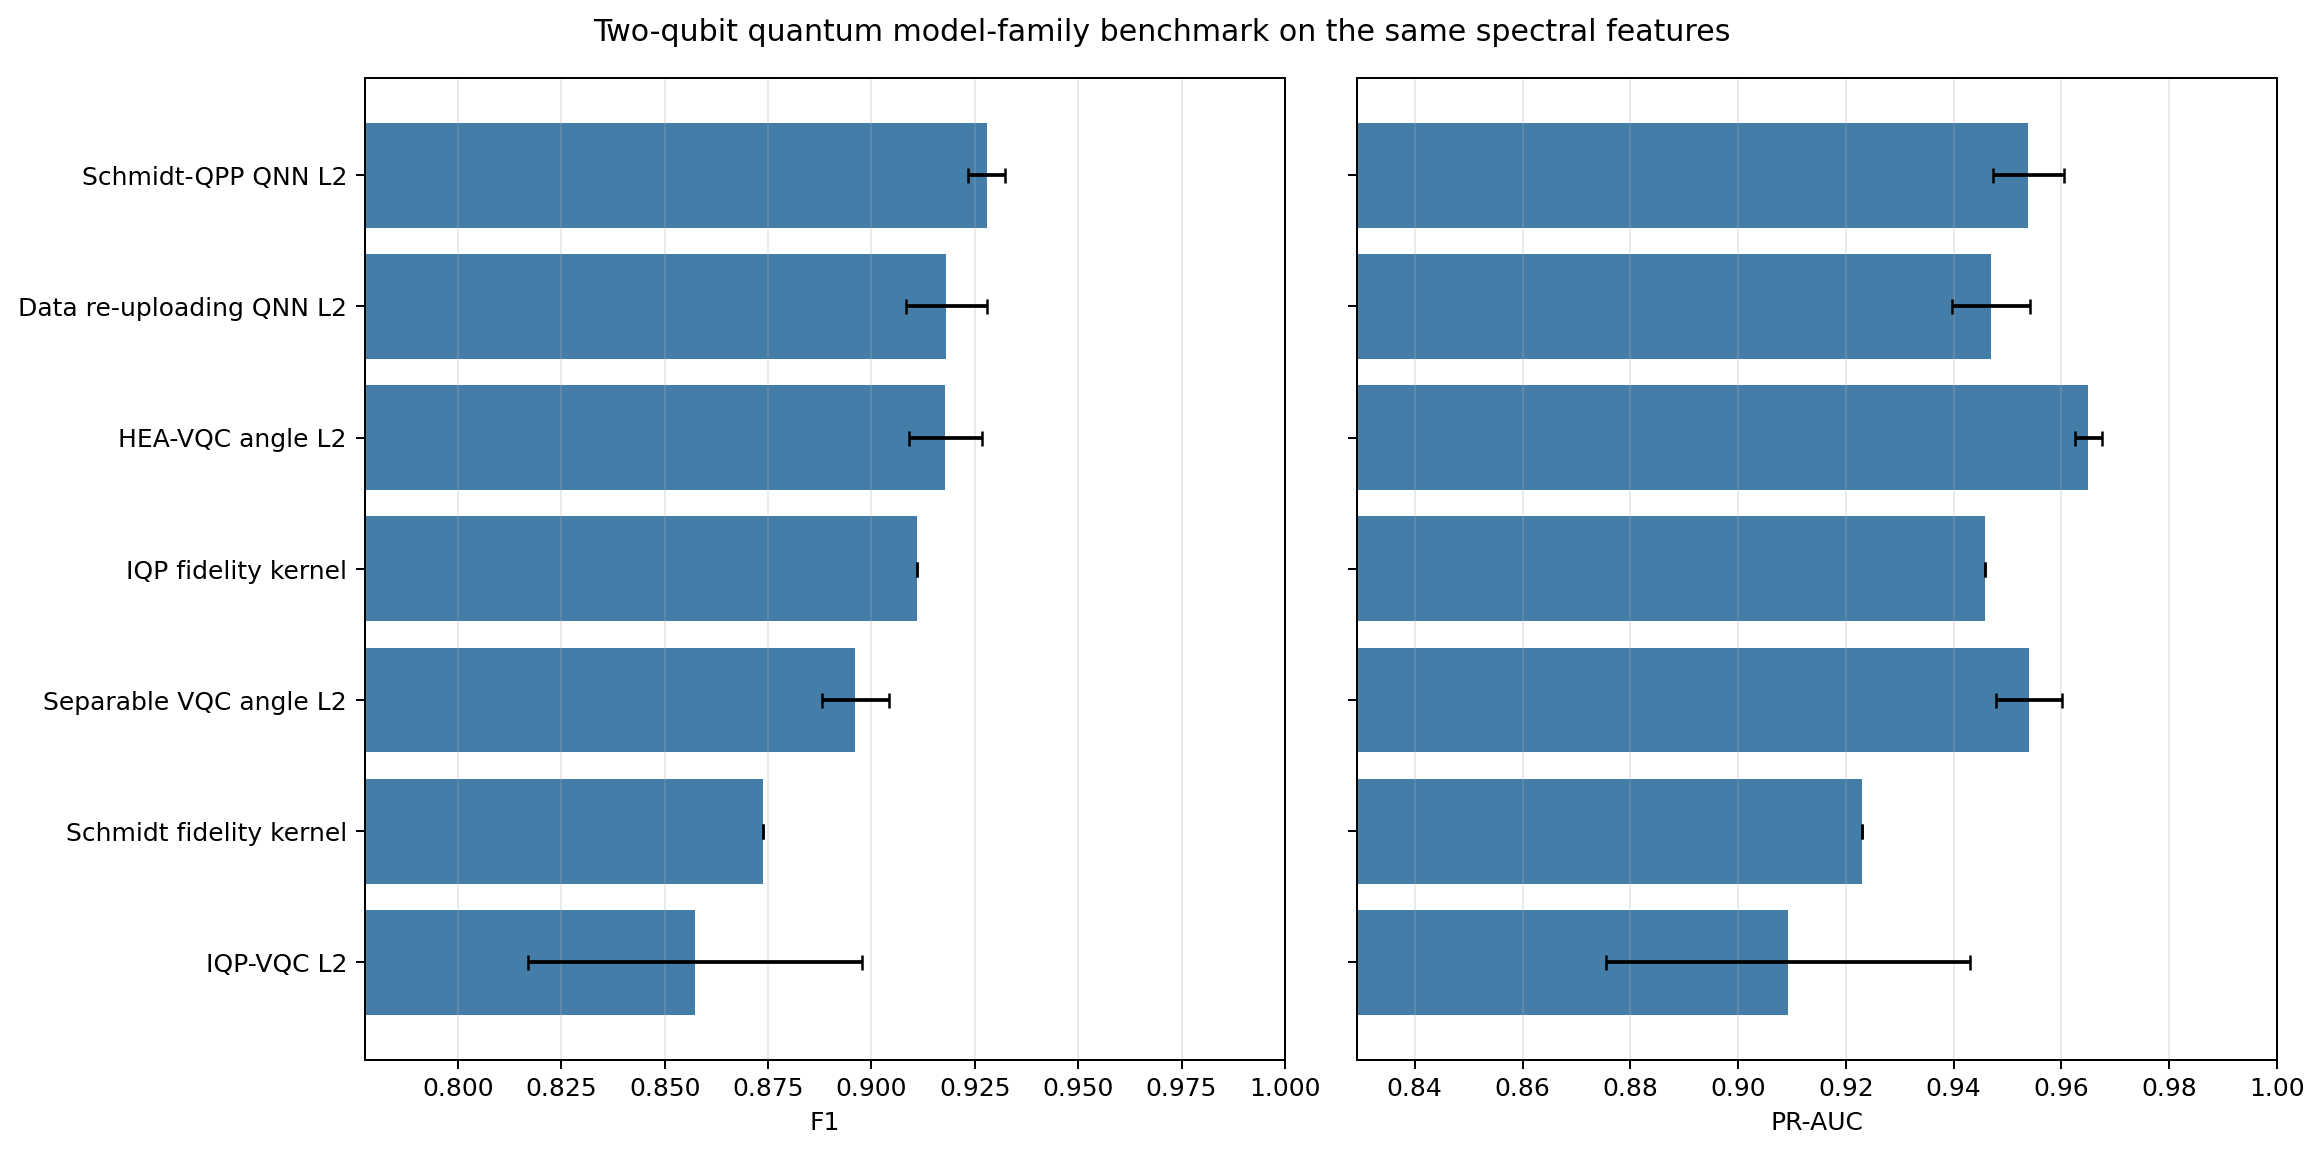
\includegraphics[width=\linewidth]{../missing_draft_figures/Figure_06_quantum_family_comparison.png}
    \caption{F1 (left) and PR-AUC (right) for the controlled two-qubit family
    comparison.  The five trainable QNN/VQC models correspond to
    Table~\ref{tab:quantum-family}; the IQP and Schmidt fidelity kernels are
    fixed-embedding quantum-kernel references and therefore have no comparable
    variational parameter count.  Error bars indicate variability across
    repeated estimates where available.}
    \label{fig:quantum-family}
\end{figure}

The Schmidt-QPP QNN obtains the highest F1,
$0.9279\pm0.0045$, indicating the best balance between precision and recall at
the validation-selected operating threshold.  The data re-uploading QNN is a
close second at $0.9181\pm0.0099$ while using 16 rather than 25 trainable
parameters---a 36\% reduction.  It therefore provides an attractive
resource--performance compromise when parameter count and hardware-oriented
circuit simplicity are important.

The ranking changes when threshold-independent quality is considered.  The
HEA-VQC achieves the highest PR-AUC, $0.9650\pm0.0025$, although its F1 is below
that of Schmidt-QPP.  Thus, Schmidt-QPP provides the strongest result at the
selected decision threshold, whereas HEA-VQC gives the best overall
precision--recall ranking across thresholds.  Reporting both metrics prevents
either behavior from being hidden by a single operating point.

The separable VQC retains a competitive PR-AUC of $0.9540\pm0.0061$ but its F1
drops to $0.8961\pm0.0080$.  This result suggests that independent one-qubit
processing can rank many samples correctly, yet is less effective at forming a
balanced decision boundary at the selected threshold.  Because the ansatzes
differ in more than entanglement alone, this gap should be interpreted as
evidence for the benefit of joint spectral modeling in the tested setting, not
as an isolated causal demonstration of quantum entanglement.  IQP-VQC records
the lowest mean scores and the largest run-to-run variation
($0.8574\pm0.0404$ F1), showing that the tested IQP-style trainable encoding is
both less accurate and less stable for these two ordered eigenvalue features.

Figure~\ref{fig:quantum-family} further shows that the two fixed
fidelity-kernel references do not dominate the best trainable circuits.  A
fixed quantum similarity geometry alone is therefore insufficient to explain
the leading results; task-adaptive variational training is important in this
benchmark.  Overall, no single family wins every criterion: Schmidt-QPP is the
preferred accuracy-oriented model, HEA-VQC provides the strongest PR-AUC, and
data re-uploading offers the clearest reduction in trainable parameters with
only a modest F1 loss.  These conclusions establish a resource-aware basis for
the noise-robustness experiments in the following section.

\subsection{Noise Robustness}
\label{sec:noise-robustness}

We next evaluate whether the clean-data decision rules remain usable after the
image distribution changes.  These experiments concern corruption of the
\emph{input images}, rather than gate or measurement noise on quantum hardware.
Unless explicitly stated otherwise, every learner is trained on clean images,
its decision threshold is selected on the clean validation split, and that
threshold is then frozen for all corrupted test sets.  Noise is applied to the
held-out test images before the original candidate centers are used to extract
new $9\times9$ patches and recompute the structure-tensor features.  The
protocol therefore measures robustness without test-time threshold
recalibration.

The evidence below comes from four deliberately separated study blocks.  The
first reproduces the original phase-coordinate QPP--QNN corruption test.  The
second is an additional matched-feature study of the earlier 5D/8D QNN
families against corresponding MLPs.  The third is a newly reconstructed,
scale-free Schmidt diagnostic designed specifically to isolate the effect of
normalizing away tensor energy.  The final block reports noise-aware adaptation
for the original phase-coordinate branch and the archived Schmidt branch.
Results are compared only within a block unless the models, inputs, and
training protocol are explicitly matched; absolute numbers from different
blocks should not be interpreted as repeated runs of one model.

In addition to absolute F1, we use the clean-relative F1 retention
\begin{equation}
    \rho_{\mathrm{F1}}(\nu)
    =\frac{\mathrm{F1}(\nu)}{\mathrm{F1}(0)},
    \label{eq:f1-retention}
\end{equation}
where $\nu$ denotes the corruption intensity.  Absolute F1 determines which
model is preferable at a given operating condition, whereas
$\rho_{\mathrm{F1}}$ separates degradation rate from clean-set accuracy.
PR-AUC is reported alongside both measures because a model can lose its fixed
operating point while still retaining useful score ordering.

\subsubsection{Gaussian and Blur Corruption}
\label{sec:gaussian-blur}

Figure~\ref{fig:qpp-corruption-response} first reports the original compact
phase-coordinate study under two levels of additive Gaussian noise, Gaussian
blur, and salt-and-pepper corruption.  Pixel-level Gaussian noise is generated
as $I'=\operatorname{clip}(I+\epsilon,0,1)$ with
$\epsilon\sim\mathcal{N}(0,\sigma^2)$.  The two-qubit QPP--QNN is particularly
stable under mild additive corruption: its F1 changes from 0.9204 on clean
images to 0.9080 at $\sigma=0.04$, corresponding to 98.7\% retention.  At
$\sigma=0.08$ it still reaches 0.8266 F1 and 0.9254 PR-AUC, retaining 89.8\%
of its clean F1.  By contrast, the one-qubit scalar model falls from 0.9131 to
0.3989 F1 at the same noise level.  The large separation at $\sigma=0.08$
shows that preserving $[\lambda_1,\lambda_2]$ as two coordinates is much more
reliable than compressing the spectrum into the single scalar
$\log(S+\epsilon)+4\eta$ under this perturbation.

The advantage is corruption dependent rather than universal.  Under blur
radius 0.9, the two-qubit model obtains 0.6797 F1: its precision remains high
at 0.9691, but recall decreases to 0.5233 because smoothing attenuates the
local gradients used by the fixed clean threshold.  The one-qubit model and
the logistic $[\log(S+\epsilon),\eta]$ control reach 0.8100 and 0.9000 F1,
respectively.  Thus, the two-coordinate circuit provides the strongest QPP
response to Gaussian perturbation, but blur remains a distinct failure mode
that cannot be summarized by a general claim of corruption invariance.

\begin{figure}[H]
    \centering
    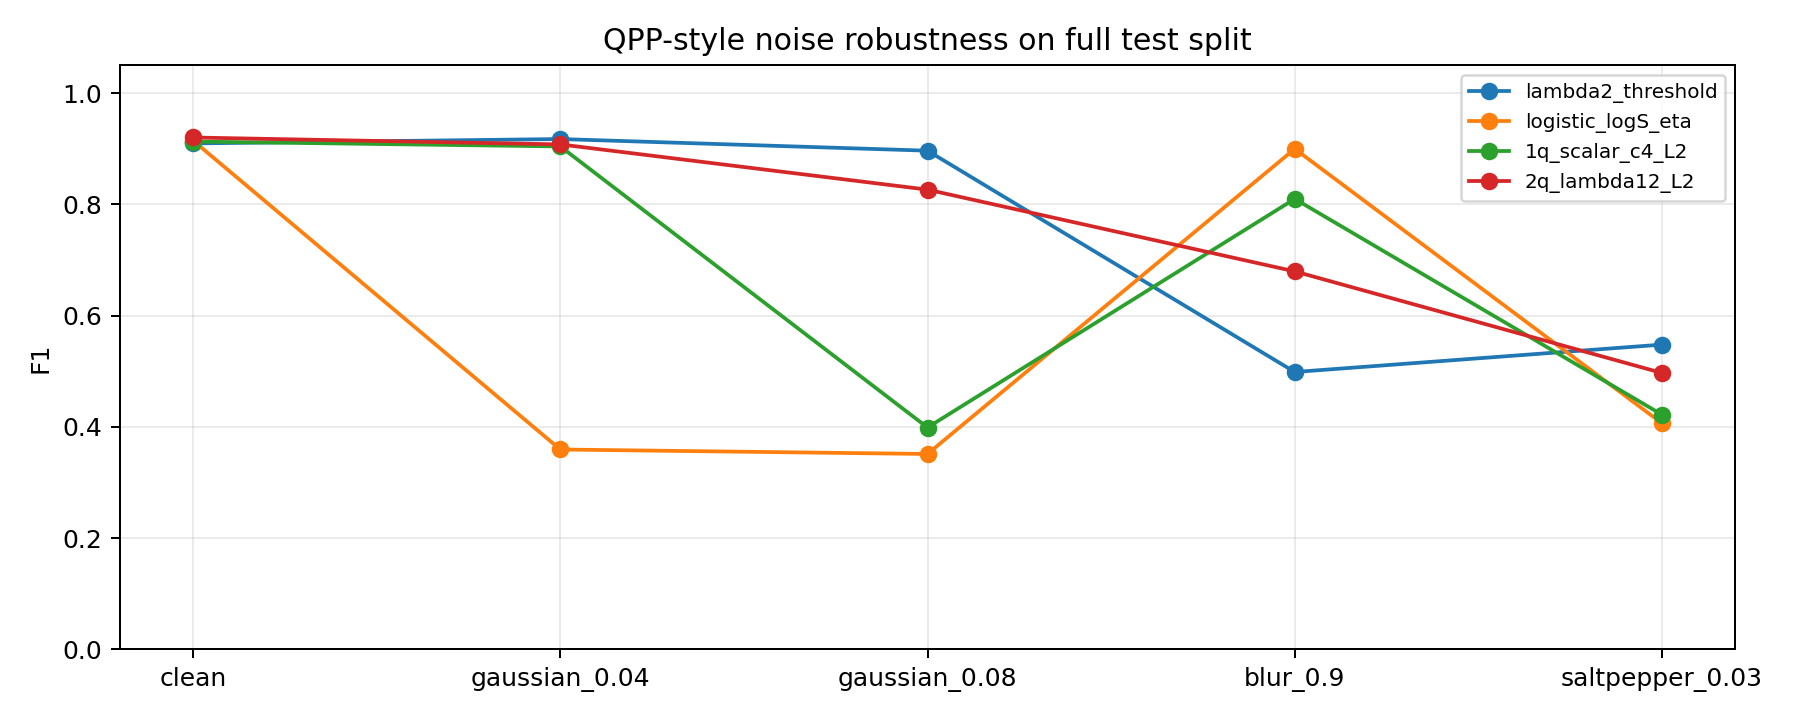
\includegraphics[width=\linewidth]{../outputs/qpp/noise/qpp_noise_robustness.png}
    \caption{Fixed-threshold F1 of the phase-coordinate QPP--QNNs and compact
    classical controls under clean, Gaussian, blur, and salt-and-pepper test
    conditions.  All thresholds are selected before corrupted test evaluation.
    The two-qubit $[\lambda_1,\lambda_2]$ model remains substantially more
    stable than the one-qubit scalar encoding at Gaussian $\sigma=0.08$.}
    \label{fig:qpp-corruption-response}
\end{figure}

\subsubsection{Extended Matched-Feature Salt-and-Pepper Sweep}
\label{sec:saltpepper-sweep}

Salt-and-pepper noise is more challenging because isolated intensity impulses
create strong local gradients and can turn background patches into apparent
keypoints.  We therefore add a separate stress test based on the earlier
feature-dimension QNN families.  This is an extension of the original
phase-coordinate experiment above, not a new noise evaluation of the same
one- or two-qubit circuit.  To compare classical and quantum learners within
this extension under matched inputs, we use a five-dimensional interface
$[I_x,I_y,\lambda_1,\lambda_2,R]$ and an eight-dimensional interface
$[I_x,I_y,I_x^2,I_y^2,I_xI_y,\lambda_1,\lambda_2,R]$.  Within each feature
dimension the QNN and MLP use the same clean train/validation/test patches, and
the noise probability is swept from $p=0$ to $p=0.15$.  Their clean scores are
therefore valid baselines for the retention calculation in this block, but are
not substitutes for the clean phase-coordinate results in
Section~\ref{sec:gaussian-blur}.

\begin{figure}[H]
    \centering
    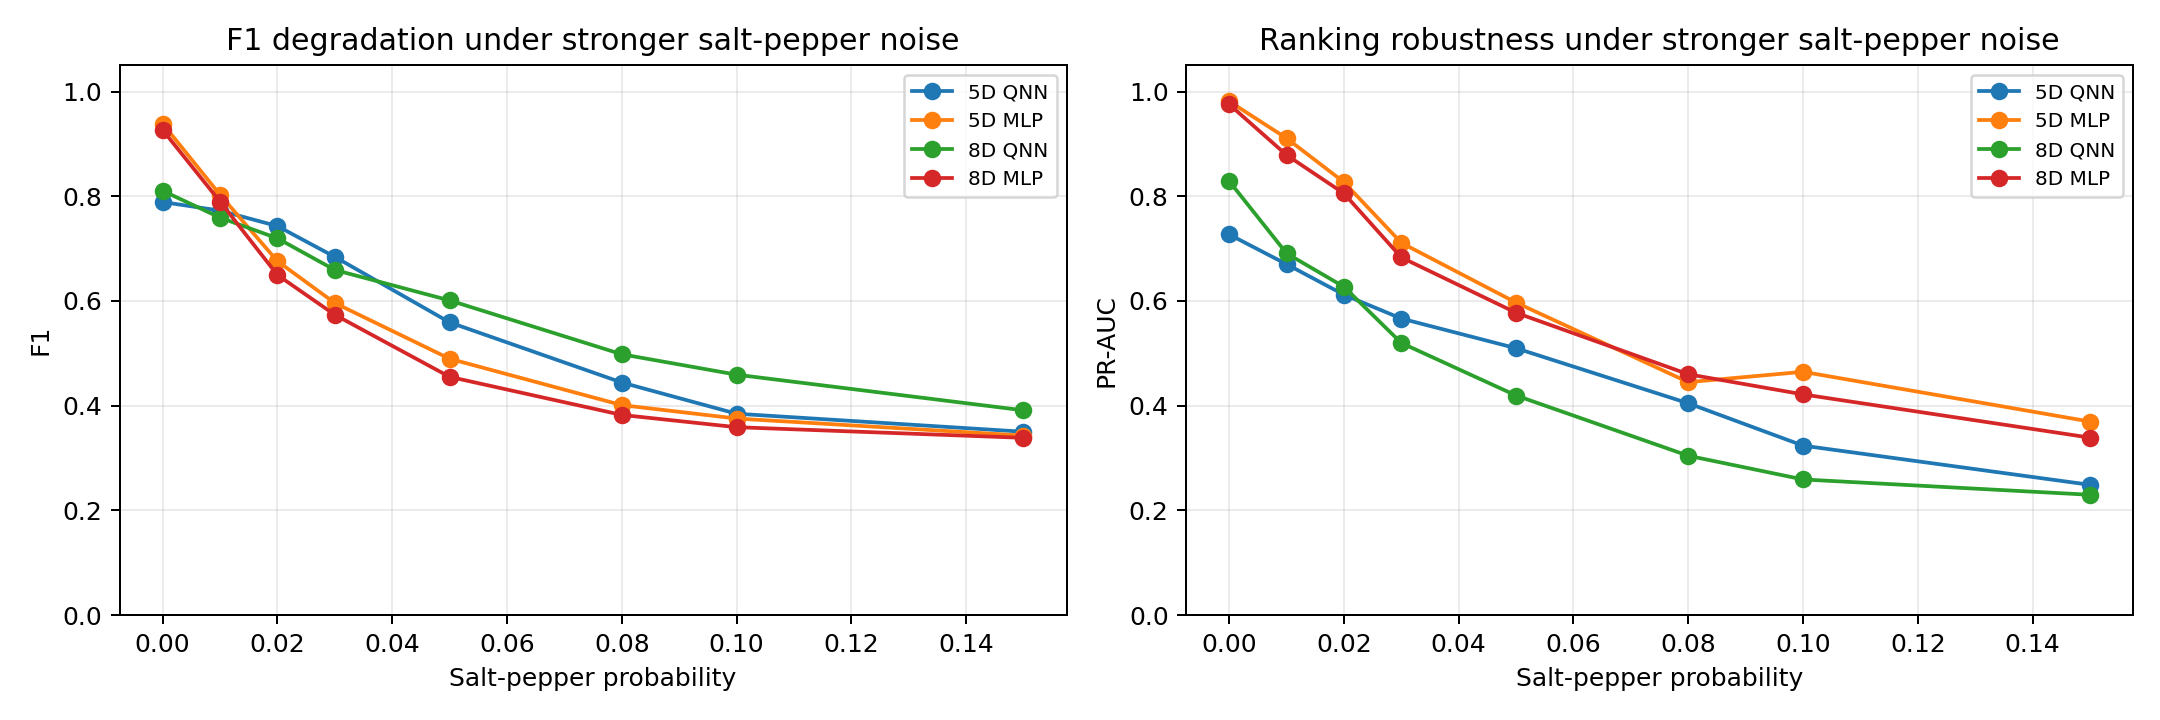
\includegraphics[width=\linewidth]{../outputs/qnn_improvement/noise_5d8d/saltpepper_sweep_5d8d.png}
    \caption{Additional matched-feature comparison of the earlier five- and
    eight-dimensional QNN/MLP families under increasing salt-and-pepper
    probability.  The left panel reports F1 at the frozen clean threshold and
    the right panel reports PR-AUC.  The QNN curves decay more slowly in
    fixed-threshold F1, whereas the MLPs retain stronger global score ranking
    over much of the sweep.}
    \label{fig:saltpepper-sweep}
\end{figure}

Figure~\ref{fig:saltpepper-sweep} reveals a crossover between clean accuracy
and corrupted operating-point stability.  The MLPs are stronger on clean
images, reaching 0.9430 and 0.9338 F1 for the 5D and 8D inputs, respectively,
compared with 0.7890 and 0.8105 for the corresponding QNNs.  At $p=0.01$ the
MLPs retain a small absolute lead.  From $p=0.02$ onward, however, both QNNs
obtain higher fixed-threshold F1 than their dimension-matched MLPs.  The common
$p=0.03$ operating point is summarized in
Table~\ref{tab:saltpepper-operating-point}.

\begin{table}[H]
    \centering
    \caption{Matched QNN/MLP performance under salt-and-pepper probability
    $p=0.03$.  Retention is defined by Eq.~\eqref{eq:f1-retention}; precision
    and PR-AUC are measured on the corrupted test set.}
    \label{tab:saltpepper-operating-point}
    \small
    \begin{tabular}{lccccc}
        \toprule
        Model & Clean F1 & Noisy F1 & F1 retention & Precision & PR-AUC \\
        \midrule
        5D QNN & 0.7890 & \textbf{0.6842} & \textbf{0.867} & \textbf{0.5482} & 0.5665 \\
        5D MLP & \textbf{0.9430} & 0.5774 & 0.612 & 0.4123 & \textbf{0.7048} \\
        8D QNN & 0.8105 & \textbf{0.6593} & \textbf{0.813} & \textbf{0.5224} & 0.5198 \\
        8D MLP & \textbf{0.9338} & 0.5611 & 0.601 & 0.3921 & \textbf{0.6775} \\
        \bottomrule
    \end{tabular}
\end{table}

At $p=0.03$, the 5D QNN exceeds the 5D MLP by 0.1068 F1 and retains 86.7\%
of its clean score, versus 61.2\% for the MLP.  The 8D QNN similarly exceeds
its MLP by 0.0982 F1 and retains 81.3\%, versus 60.1\%.  The MLPs maintain
recall above 0.96 but their precision falls to 0.4123 and 0.3921, indicating
that impulse-induced false positives overwhelm the clean-calibrated decision
threshold.  The QNNs trade a modest amount of recall for precision above 0.52
and consequently obtain the better deployed F1 without recalibration.

Over the complete $p=0$ to $p=0.15$ sweep, F1 decreases by 0.4387 for the 5D
QNN and 0.4193 for the 8D QNN, compared with drops of 0.6020 and 0.5930 for
the corresponding MLPs.  Nevertheless, the right panel of
Fig.~\ref{fig:saltpepper-sweep} shows that MLP PR-AUC remains higher over most
noise levels.  The supported advantage is therefore precise: the QNNs provide
a more stable \emph{fixed clean-calibrated operating point} under impulsive
corruption, rather than a uniformly superior ranking at every possible
threshold.

\subsubsection{Reconstructed Scale-Free Schmidt Diagnostic}
\label{sec:representation-robustness}

The preceding results use feature sets that retain gradient magnitude and
tensor-energy information.  We next isolate what happens when the quantum
state contains only the normalized Schmidt spectrum.  Because the training
script and checkpoint associated with the original archived Schmidt noise
table are not available, the following experiment is explicitly treated as a
new reconstruction rather than a replication of that table.  The matched
diagnostic compares a 25-parameter scale-free Schmidt reconstruction with two
21-parameter TinyMLPs.  The first MLP receives the raw ordered eigenvalues
$[\lambda_1,\lambda_2]$, while the second receives exactly the normalized
spectrum $[\mu_1,\mu_2]$ encoded by the Schmidt state, where
$\mu_i=\lambda_i/(\lambda_1+\lambda_2)$.  Results are averaged over five
training seeds and, for nonzero corruption, three independently generated
noise instances per training seed.

\begin{table}[H]
    \centering
    \caption{F1 in the independently reconstructed, representation-matched
    robustness diagnostic.  The raw-spectrum MLP retains tensor energy,
    whereas the scale-free Schmidt model and the $\mu_{12}$ MLP are invariant
    to a common rescaling of both eigenvalues.}
    \label{tab:schmidt-noise-diagnostic}
    \small
    \begin{tabular}{lccc}
        \toprule
        Test condition & Scale-free Schmidt & MLP $\lambda_{12}$ & MLP $\mu_{12}$ \\
        \midrule
        Clean & 0.8738 & \textbf{0.9259} & 0.8738 \\
        Gaussian $\sigma=0.01$ & 0.3586 & \textbf{0.9250} & 0.3586 \\
        Gaussian $\sigma=0.04$ & 0.3542 & \textbf{0.9147} & 0.3542 \\
        Salt-and-pepper $p=0.03$ & 0.3730 & \textbf{0.4843} & 0.3730 \\
        \bottomrule
    \end{tabular}
\end{table}

The scale-free Schmidt reconstruction and the representation-matched
$\mu_{12}$ MLP produce identical
F1, precision, and recall throughout both noise sweeps, with only numerical
round-off differences in PR-AUC.  In contrast, the raw-spectrum MLP is far
more stable under Gaussian noise.  The reason is visible in the feature
statistics.  For clean negative patches the median tensor energy
$S=\lambda_1+\lambda_2$ and median $\mu_2$ are both zero.  At
$\sigma=0.01$, the negative-patch median energy is still only 0.0141, compared
with 5.1257 for positive patches, but its median $\mu_2$ rises to 0.4202,
slightly above the positive median of 0.3746.  Normalization therefore makes
weak, nearly isotropic noise resemble a genuine corner while discarding the
small energy that would identify it as background.

This diagnostic does not imply that every quantum encoding is noise sensitive;
it identifies a boundary of this reconstructed scale-free representation.  In
particular, its values must not be substituted for either the clean Schmidt
family comparison in Table~\ref{tab:quantum-family} or the archived Schmidt
noise-aware summary below, because those results use different circuit and
training implementations.  The diagnostic instead shows why the positive
5D/8D and phase-coordinate results should be attributed to the joint choice of
retained geometric information and classifier, not to quantumness alone.  It
further motivates an energy-aware Schmidt interface,
such as $[\log(S+\epsilon),\mu_2]$, an explicit trace floor, or a classical
energy gate alongside the quantum readout.

\subsubsection{Noise-Aware Training}
\label{sec:noise-aware-training}

Finally, we return to the original study and ask whether its difficult
salt-and-pepper operating points can be recovered by exposing the QPP--QNNs to
representative corruptions during optimization.  For the reproducible
phase-coordinate run, clean-only training uses 4,500 patches.  The noise-aware
run augments them with Gaussian
$\sigma\in\{0.04,0.08\}$, blur radius 0.9, and salt-and-pepper $p=0.03$
versions, giving 22,500 training instances.  The corrupted images are passed
through the complete feature-extraction pipeline rather than perturbing the
already computed feature vectors.  The initial study also archives summary
metrics for a separate Schmidt-QPP branch.  Those Schmidt values are reported
as their own row pair and are not combined with the reconstructed scale-free
diagnostic in Section~\ref{sec:representation-robustness}.

\begin{table}[H]
    \centering
    \caption{Within-branch recovery on salt-and-pepper $p=0.03$ before and
    after noise-aware training.  The phase-coordinate row is reproduced from
    the available run outputs; the Schmidt row records the archived summary
    from the initial study.}
    \label{tab:noise-aware-training}
    \small
    \begin{tabular}{lcccc}
        \toprule
        Model branch & F1 clean & F1 adapted & PR-AUC clean & PR-AUC adapted \\
        \midrule
        Phase-coordinate 2q & 0.5448 & \textbf{0.7307} & 0.4857 & \textbf{0.7712} \\
        Archived Schmidt-QPP & 0.5064 & \textbf{0.7128} & 0.5530 & \textbf{0.8146} \\
        \bottomrule
    \end{tabular}
\end{table}

\begin{figure}[H]
    \centering
    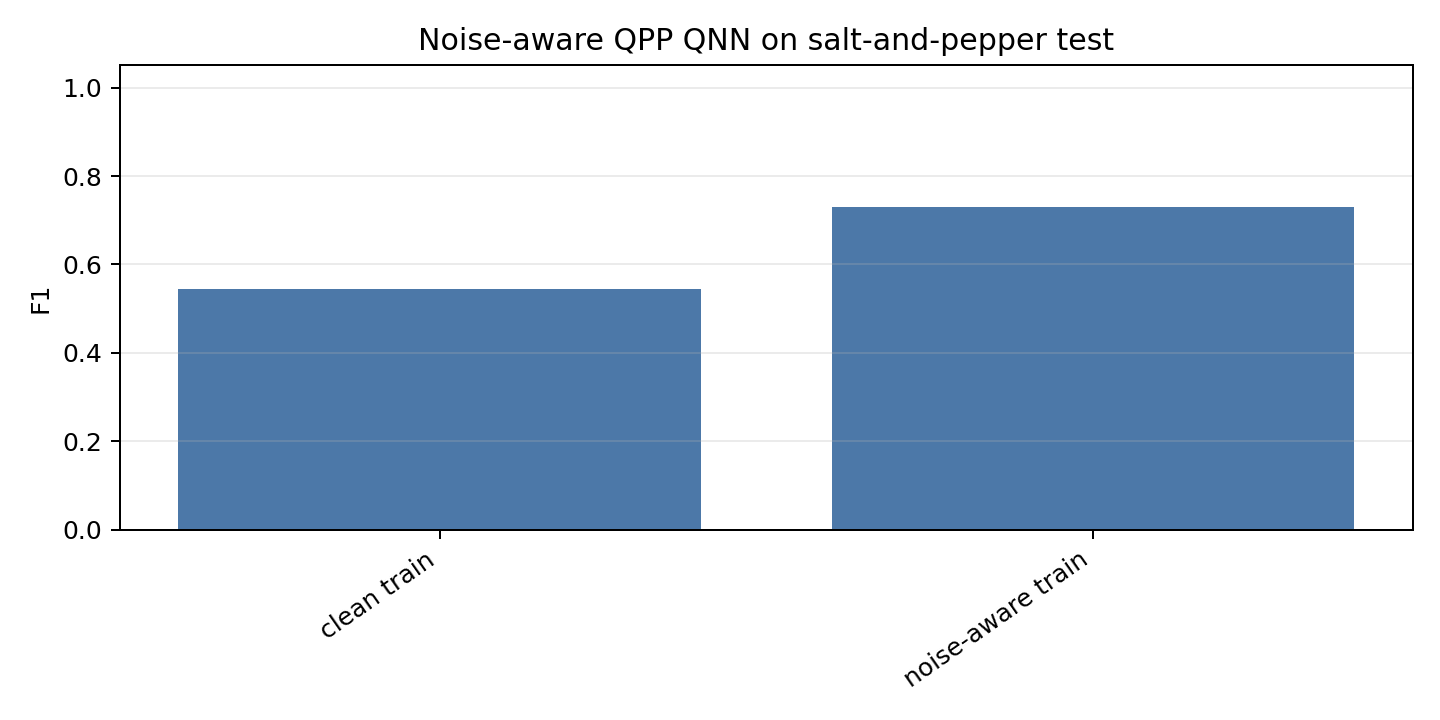
\includegraphics[width=0.58\linewidth]{../outputs/qpp/noise_aware/qpp_noise_aware_results.png}
    \caption{Recovery of the phase-coordinate two-qubit QPP--QNN under
    salt-and-pepper $p=0.03$.  This figure visualizes the first row of
    Table~\ref{tab:noise-aware-training}; the archived Schmidt branch is kept
    numerically separate in the second row.}
    \label{fig:noise-aware-training}
\end{figure}

For the phase-coordinate branch, noise-aware training increases F1 by 0.1859,
from 0.5448 to 0.7307, which is a 34.1\% relative improvement.  PR-AUC rises
by 0.2855, from 0.4857 to 0.7712.  The available detailed output shows that the
dominant operating-point change is the precision increase from 0.3768 to
0.6407: although recall decreases from 0.9833 to 0.8500, the model suppresses
enough impulse-induced false positives to achieve a substantially better
precision--recall balance.

The archived Schmidt branch exhibits the same qualitative adaptation pattern:
F1 increases by 0.2064, from 0.5064 to 0.7128, and PR-AUC increases by 0.2616,
from 0.5530 to 0.8146.  These summary values support the original observation
that impulse noise requires augmentation, but they are not evidence that the
archived Schmidt implementation and the new scale-free reconstruction behave
identically.  Moreover, both noise-aware branches use augmented training data
and neither has a matched noise-aware MLP in this study.  The result therefore
demonstrates recoverability of each QPP--QNN branch rather than a matched
classical advantage.

Taken together, the separated experiments establish a conditional robustness
result.  In the original phase-coordinate study, the two-qubit spectral
representation is substantially more stable than its one-qubit compression
under Gaussian noise.  In the additional matched-feature study, the 5D/8D
QNNs maintain a more stable clean-calibrated operating point than the matched
MLPs under moderate salt-and-pepper corruption.  The newly
reconstructed scale-free diagnostic then shows that this behavior is
representation dependent: removing the tensor-energy cue can eliminate
robustness even when the downstream circuit is trainable.  Finally, the
phase-coordinate and archived Schmidt branches both improve substantially with
noise-aware training.  Robust quantum-edge inference should therefore be
understood as the joint design of geometric representation, circuit
architecture, and corruption-aware training, rather than as an automatic
consequence of using a quantum classifier.

\subsection{Ablation Studies}

\subsubsection{Circuit Depth}

\subsubsection{Entangling Patterns}

\subsubsection{Observable Readout}

\subsection{Cross-Domain Transfer}

\subsubsection{Three-Dimensional Point Covariance}

\subsubsection{Multichannel PSD Classification}

\subsection{Quantum Hardware Execution}

\subsubsection{Backend and Circuit Configuration}

\subsubsection{Readout Correction and Hardware Results}

\end{document}
